\documentclass{standalone}
\usepackage{pgfplots}
\usetikzlibrary{shapes.geometric, intersections, calc}
\pgfplotsset{compat=1.7}

\begin{document}
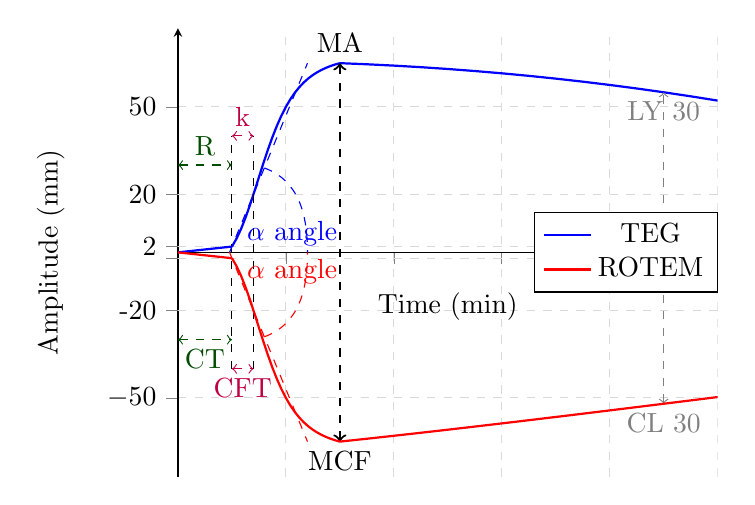
\begin{tikzpicture}

\tikzset{
    myarrow/.style={
        sloped,
        isosceles triangle,
        anchor=apex,
        fill=black,
        inner sep=2pt
    }
}

\makeatletter
\def\parsenode[#1]#2\pgf@nil{%
    \tikzset{label node/.style={#1}}
    \def\nodetext{#2}
}

\tikzset{
    add node at x/.style 2 args={
        name path global=plot line,
        /pgfplots/execute at end plot visualization/.append={
                \begingroup
                \@ifnextchar[{\parsenode}{\parsenode[]}#2\pgf@nil
            \path [name path global = position line #1-1]
                ({axis cs:#1,0}|-{rel axis cs:0,0}) --
                ({axis cs:#1,0}|-{rel axis cs:0,1});
            \path [xshift=1pt, name path global = position line #1-2]
                ({axis cs:#1,0}|-{rel axis cs:0,0}) --
                ({axis cs:#1,0}|-{rel axis cs:0,1});
            \path [
                name intersections={
                    of={plot line and position line #1-1},
                    name=left intersection
                },
                name intersections={
                    of={plot line and position line #1-2},
                    name=right intersection
                },
                label node/.append style={pos=1}
            ] (left intersection-1) -- (right intersection-1)
            node [label node]{\nodetext};
            \endgroup
        }
    },
    add node at y/.style 2 args={
        name path global=plot line,
        /pgfplots/execute at end plot visualization/.append={
                \begingroup
                \@ifnextchar[{\parsenode}{\parsenode[]}#2\pgf@nil
            \path [name path global = position line #1-1]
                ({axis cs:0,#1}-|{rel axis cs:0,0}) --
                ({axis cs:0,#1}-|{rel axis cs:1,1});
            \path [yshift=1pt, name path global = position line #1-2]
                ({axis cs:0,#1}-|{rel axis cs:0,0}) --
                ({axis cs:0,#1}-|{rel axis cs:1,1});
            \path [
                name intersections={
                    of={plot line and position line #1-1},
                    name=left intersection
                },
                name intersections={
                    of={plot line and position line #1-2},
                    name=right intersection
                },
                label node/.append style={pos=1}
            ] (left intersection-1) -- (right intersection-1)
            node [label node] {\nodetext};
            \endgroup
        }
    }
}
\makeatother
    \begin{axis}[
        axis x line=middle,
        axis y line=middle,
        x tick label style={/pgf/number format/fixed,
                            /pgf/number format/fixed zerofill,
                            /pgf/number format/precision=1},
        y tick label style={/pgf/number format/fixed,
                            /pgf/number format/fixed zerofill,
                            /pgf/number format/precision=0},
        grid = major,
        grid style={dashed, gray!30},
	extra y ticks={2, 20, -2, -20},
extra y tick labels={2, 20, , -20},
        xmin=0,     % start the diagram at this x-coordinate
        xmax= 50,    % end   the diagram at this x-coordinate
        ymin= -77,     % start the diagram at this y-coordinate
        ymax= 77,   % end   the diagram at this y-coordinate
        %axis background/.style={fill=white},
    	  x label style={at={(axis description cs:0.5,-0.1)},anchor=north},
	  y label style={at={(axis description cs:-0.1,.5)},rotate=90,anchor=south},
	  xticklabels={},
	 ylabel near ticks,
	xlabel near ticks,
        xlabel=Time (min),
        ylabel=Amplitude (mm),
        tick align=outside,
        enlargelimits=false,
	legend style={at={(axis cs:33,0)},anchor=west}]

	\addlegendimage{blue, thick}
	\addlegendentry{TEG};
	\addlegendimage{red, thick}
	\addlegendentry{ROTEM};

	\addplot[blue, thick, domain=0:5] {0.4*x};
	\addplot[blue, thick, domain=5:15] {68.01378 + (-4.146473 - 68.01378)/(1 + (x/8.028773)^5.012703)};
	\addplot[blue, thick, domain=15:75] {(65.91032 - -301.9906)/(1 + (x/206.966)^2.285876) - 301.9906};

	\draw[black,thin,dashed] (axis cs: 5,-40) -- (axis cs: 5, 40);
	\draw[black!70!green,thin,dashed,thin,dashed, <->] (axis cs: 0, 30) -- (axis cs: 2.5, 30) node[above, black!70!green,thin,dashed]{R} -- (axis cs: 5,30);
	\draw[black,thin,dashed] (axis cs: 7,-40) -- (axis cs: 7, 40);
	\draw[purple,thin,dashed, <->] (axis cs: 5, 40) -- (axis cs: 6, 40) node[above, purple]{k} -- (axis cs: 7,40);
	\addplot[blue, thin, dashed, domain=4.77:12] {9*x - 43} node[right, blue, pos=0.1]{$\alpha$ angle};
	\draw[blue, thin, dashed] (axis cs: 8, 29) node (a){} to[out= -20, in=90] (axis cs: 12, 0) node (b){};


	\draw[black,thick,dashed, <->] (axis cs: 15,-65) node[below, black]{MCF}-- (axis cs: 15, 65) node[above, black]{MA};
	\draw[black!70!green,thin,dashed,thin,dashed, <->] (axis cs: 0, -30) -- (axis cs: 2.5, -30) node[below, black!70!green,thin,dashed]{CT} -- (axis cs: 5,-30);
	\draw[gray,thin,dashed, <->] (axis cs: 45,-52) node[below,gray]{CL 30} -- (axis cs: 45, 55) node[below,gray]{LY 30};
	\draw[purple,thin,dashed, <->] (axis cs: 5, -40) -- (axis cs: 6, -40) node[below, purple]{CFT} -- (axis cs: 7,-40);

	\addplot[red, thin, dashed, domain=4.77:12] {43 - 9*x} node[right, red, pos=0.1]{$\alpha$ angle};
	\draw[red, thin, dashed] (axis cs: 8, -29) node (a){} to[out= 20, in=-90] (axis cs: 12, 0) node (b){};


	\addplot[red, thick, domain=0:5] {-0.4*x};
	\addplot[red, thick, domain=5:15] {-68.01378 - (-4.146473 - 68.01378)/(1 + (x/8.028773)^5.012703)};
	\addplot[red, thick, domain=15:75] {245.7324 + (-69.81802 - 245.7324)/(1 + (x/444.6476)^1.229355)};



\end{axis}

\end{tikzpicture} 
\end{document}